\chapter{Security of network applications}
\section{Standard situation}
The standard situation for an ordinary network application is very \textbf{negative}, since most of the systems implement very \textbf{weak authN mechanism} that typically rely on \texttt{username} and \texttt{password}, which can lead to:
\begin{itemize}
    \item Password Snooping
    \item IP Spoofing 
\end{itemize}
Even if \textbf{stronger authN mechanism} is implemented, there are still problems with data:
\begin{itemize}
    \item Data Snooping/Forging
    \item Shadow Server/MITM
    \item Replay and Filtering attacks
\end{itemize}
So to resolve these problems, we can use two different approaches: \textbf{Channel Security} and \textbf{Message/Data Security}.

\section{Channel Security}
\begin{minipage}{0.7\textwidth}
%	\vspace{-0.5cm}
Channel Security implements a secure connection between two nodes. To achieve this, before the start of the communication, the two nodes need to negotiate the \texttt{algorithms}, \texttt{parameters} and \texttt{keys} to protect the whole traffic that will be sent through the communication channel.
\end{minipage} 
\hspace{0.5cm}
\begin{minipage}{0.3\textwidth}
    \centering
    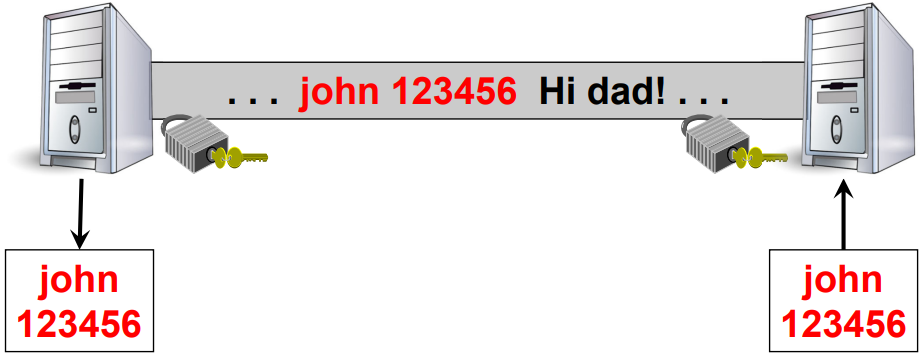
\includegraphics[width=\textwidth]{/home/lorenzo/Notes/Information System Security/images/Screenshot from 2024-12-22 13-22-37.png}
\end{minipage}
\noindent
Since all this features are negotiated \textbf{before transmitting data}, we ensure:
\begin{itemize}
    \item \textbf{Single} or \textbf{mutual authN}
    \item \textbf{Data integrity}
    \item \textbf{Data confidentiality}
\end{itemize}
Channel Security is very easy to implement because it requires no (or small) modification of applications. Since this features are also negotiated \textbf{automatically} we cannot have \textbf{non-repudation}.\\
\\
\textcolor{red}{\textbf{N.B.}} The \textbf{main issue} with Channel Security is that its security properties are provided \textbf{only} during the transit \textbf{inside} the communication channel. So data in \textbf{not} protected when it's located at the end-user. 

\section{Message/Data security}
\begin{minipage}{0.6\textwidth}
%	\vspace{-0.5cm}
It applies protection \textbf{only} when it's needed. This means that data is \textbf{individually} protected by wrapping it into a \textbf{secure container}. Data (not the channel) ensures the following security properties:
\begin{itemize}
    \item \textbf{Single authN, not mutual} because features are \textbf{not negotiated}
    \item \textbf{Data integrity}
    \item \textbf{Data confidentiality}
\end{itemize}
\end{minipage} 
\hspace{0.5cm}
\begin{minipage}{0.4\textwidth}
    \centering
    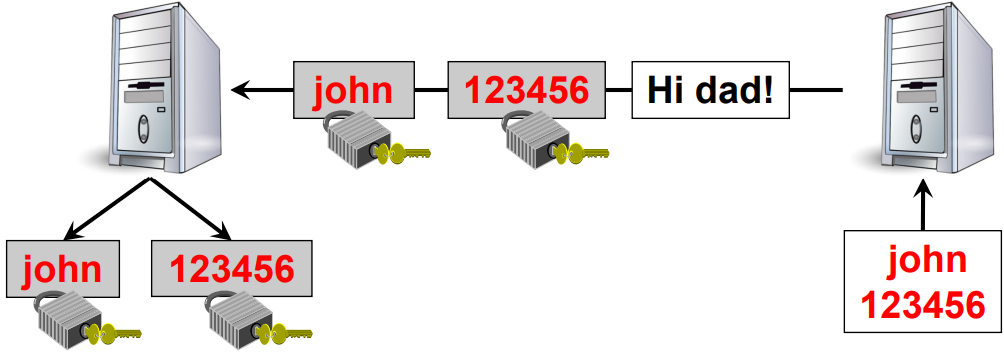
\includegraphics[width=\textwidth]{/home/lorenzo/Pictures/Screenshots/Screenshot from 2024-12-22 13-44-53.png}
\end{minipage}
\noindent
\newline
\\If protection is applied \textbf{voluntary} and \textbf{explicity} by the user, we can have \textbf{non-repudation}. Message/Data Security requires modification to application.
\newpage
\section{Different implementation}
\texttt{Channel Security} and \texttt{Message/Data Security} can be \textbf{combined} in order to get the \textbf{benefits} of both. These security concepts can be  implemented in two different way:
\\
\newline
\begin{minipage}{0.5\textwidth}
    \subsubsection{Security Internal to Applications}
    \begin{center}
        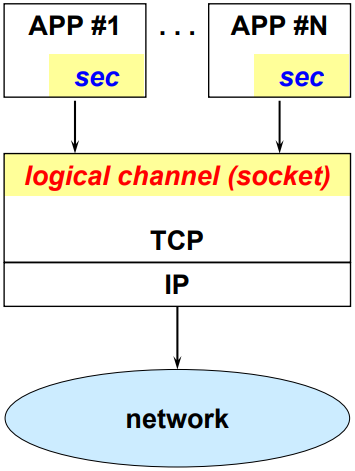
\includegraphics[width=0.3\textwidth]{/home/lorenzo/Notes/Information System Security/images/Screenshot from 2024-12-22 15-33-07.png}
    \end{center}
    In this approach \textbf{each application implements security internally}. The common part is limited to the communication channels (socket). They could be:
    \begin{itemize}
        \item  \textbf{Possible implementation errors} (implementing security protocols is not simple)
        \item Does not guarantee interoperability (-> security specification could be different between applications)
    \end{itemize}
    \textcolor{red}{\textbf{N.B.}} \textbf{Communication channels} are the \textbf{only} common part between the various application application and are used to exchange information.
\end{minipage} 
\hspace{0.5cm}
\begin{minipage}{0.5\textwidth}
    \vspace{-1cm}
    \subsubsection{Security External to Applications}
    \begin{center}
        \centering
        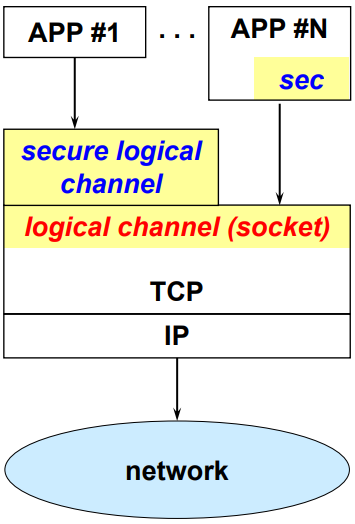
\includegraphics[width=0.3\textwidth]{/home/lorenzo/Notes/Information System Security/images/Screenshot from 2024-12-22 16-57-52.png}
    \end{center}
    A \textbf{Secure Socket} is created on top of the already existing "normal" socket, effectively creating a \textbf{new level} called \textbf{Secure Session Level (SSL)}. The Secure Socket implements all the security functions and can be used by any application that wants to communicate in a secure way. Thanks to \textbf{SSL} we can: 
    \begin{itemize}
        \item Simplify the work of application developer
        \item Avoid implementation errors
    \end{itemize}
\end{minipage}
\newline
\\
\noindent{\color{gray!50}\rule{\textwidth}{0.5pt}}
\section{TLS (Transport Layer Security)}
Originally known as \textbf{SSL}, \textbf{TLS} is a \textbf{network/session level protocol} which is capable of creating \textbf{secure transport channles} that grants:
\begin{itemize}
    \item peer authentication
    \item message confidentiality
    \item message authentication and integrity
    \item protection against replay and filtering attacks
\end{itemize}
It's easily applicable to all protocols based on \textbf{TCP}, such as HTTP, SMPT, NNTP, FTP, TELNET, \dots (e.g. HTTP (https://....) = 443/TCP).    
\begin{quotebox-yellow}{Beware}
        HTTPS is not a protocol, it's a combination of HTTP over TLS. 
\end{quotebox-yellow}
\begin{quotebox-red}{Beware}
    The current version of TLS is \textbf{TLS-1.3} and nowadays everything that uses a version \textbf{older than TLS-1.2} is considered \textbf{insecure and deprecated}.
\end{quotebox-red}

\begin{figure}[H]
    \centering
    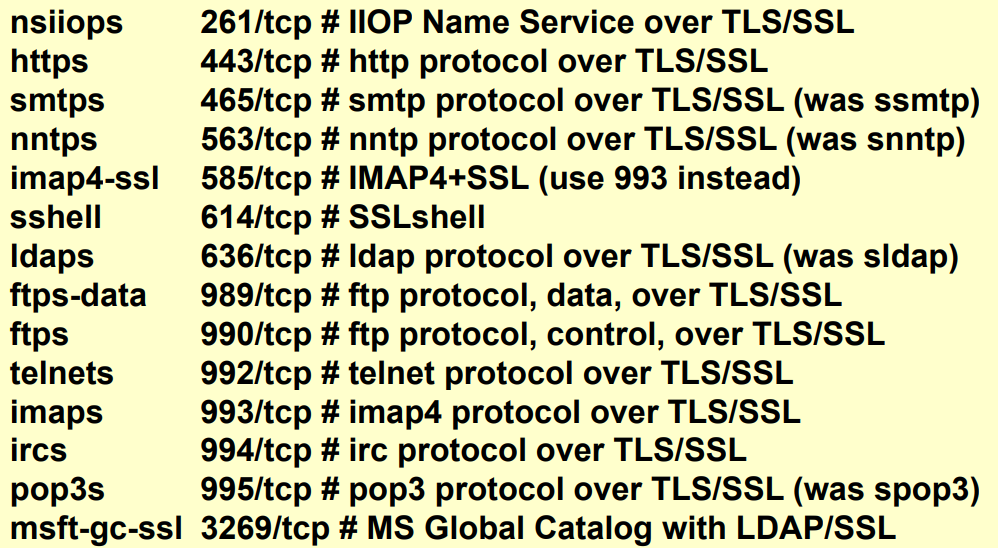
\includegraphics[width=0.4\textwidth]{/home/lorenzo/Notes/Information System Security/images/Screenshot from 2024-12-22 17-24-59.png}
    \caption{Official Ports for TLS/SSL Applications}
\end{figure}

\subsection{TLS - AuthN and Integrity}
\textbf{Peer AuthN} is performed \textbf{always at channel setup}:
\begin{itemize}
    \item The server must be authenticated (mandatory). Sends its public key (X.509 certificate) and responds to an implicit asymmetric challenge.
    \item The client can authenticate itself (optional): with public key, X.509 certificate and explicit challenge. 
\end{itemize}
For \textbf{authN} and \textbf{integrity} of \textbf{data}, TLS uses:
\begin{itemize}
    \item A Keyed-Digest (SHA-1 or better).
    \item An implicit MID to \textbf{avoid} Replay and Filtering attacks.
\end{itemize}
\subsection{TLS - Confidentiality}
\textbf{Data confidentiality} is granted by TLS in the following way:
\begin{enumerate}
    \item The client generates a session key used for symmetric encryption of data (using RC4, 3DES, IDEA, AES, or ChaCha20). 
    \item The session key is \textbf{exchanged} with the server via Asymmetric cryptography (using RSA or DH).
\end{enumerate}
\textcolor{red}{\textbf{N.B.}} Authentication is available in TLS 1.2, while is mandatory in TLS 1.3. 

\subsection{TLS Handshake Protocol}
\begin{minipage}{0.6\textwidth}
%	\vspace{-0.5cm}
    The \textbf{Handshake Protocol} is used by TLS to perform \textbf{channel setup}, let's see an example:
    \begin{enumerate}
        \item The browser (\textbf{client} \textbf{C}) initiates a connection to the \textbf{web server} (\textbf{S}) by requesting the website
        (www.polito.it) over HTTPS.
        \item \textbf{C} and \textbf{S} discuss about the security configuration. They should both agree to use the \textbf{strongest common algorithms}.
        \item The \textbf{S} sends its certificate to \textbf{C} to prove its identity. The certificate includes the server’s public key and the domain name.\\
        3b) \textbf{S} will then respond to an Asymmetric CRA sent by the \textbf{C} (This is part of the handshake to confirm (implicitly)
        the server’s identity.)
        \item (Optional) \textbf{S} may require (explicitly) a client certificate to verify
        the user’s identity.
        \item \textbf{Key exchange} is performed.
        \item Finally the \textbf{Secure TLS Channel} is opened and available to exchange data. 
    \end{enumerate}
\end{minipage} 
\hspace{0.1cm}
\begin{minipage}{0.5\textwidth}
    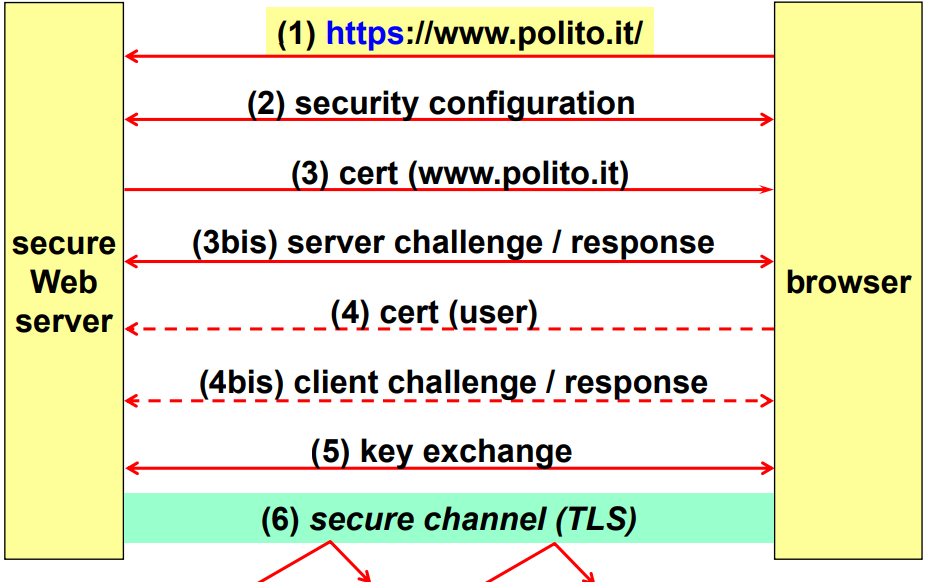
\includegraphics[width=0.9\textwidth]{/home/lorenzo/Notes/Information System Security/images/Screenshot from 2024-12-22 17-53-44.png}
\end{minipage}
